\documentclass[a4paper,11pt]{article}

\usepackage[utf8]{inputenc}
\usepackage[T1]{fontenc}
\usepackage{geometry}
\geometry{margin=2.2cm}
\usepackage{xcolor}
\usepackage{graphicx}
\graphicspath{{figures/}}
\usepackage{tikz}
\usetikzlibrary{calc}
\usepackage{everypage}
\usepackage{amsmath}
\usepackage{amssymb}
\usepackage{booktabs}
\usepackage{caption}
\usepackage{float}
\usepackage[colorlinks=true,linkcolor=blue,urlcolor=blue]{hyperref}

\setlength{\parskip}{0.6em}
\setlength{\parindent}{0pt}

\definecolor{bordercolor}{RGB}{68,94,114}

\AddEverypageHook{%
  \begin{tikzpicture}[remember picture, overlay]
    \draw[line width=4pt, color=bordercolor]
      ($(current page.south west) + (1cm,1cm)$) rectangle
      ($(current page.north east) - (1cm,1cm)$);
  \end{tikzpicture}%
}

\begin{document}

\begin{titlepage}
\thispagestyle{empty}
\centering
\vspace*{3cm}
{\Huge\bfseries Loss Given Default Model\\\bigskip
\LARGE A Retail LGD Scorecard with Downturn Adjustment
\par}
\vspace{1.5cm}
{\Large Magnus Foldeström\par}
\vfill
\end{titlepage}

\section{What this project does}

Loss Given Default (LGD) is the fraction of exposure that is lost when
a borrower defaults, after all recoveries. It is one of the three
components of the expected loss identity used across Basel IRB and
IFRS 9:
$$\mathrm{EL} = \mathrm{PD} \cdot \mathrm{LGD} \cdot \mathrm{EAD}.$$

This project builds a retail LGD scorecard on a synthetic panel of
$\sim$15{,}000 defaulted facilities across mortgage, auto, personal
secured, and unsecured collateral, spanning ten origination vintages
(2019H1--2023H2). The model estimates realised LGD from facility and
borrower features, calibrates by collateral bucket, and derives a
downturn-adjusted LGD as required by Basel IRB.

\section{Data}

Each row is one defaulted facility observed to workout resolution.
Features cover collateral type, exposure at default, loan-to-value at
default, days past due at workout start, workout duration, borrower
age and employment status, and vintage-level macro context
(unemployment, house-price index growth). The target is realised LGD
drawn from a Beta distribution whose mean depends on the features.

\begin{table}[H]
\centering
\begin{tabular}{l r r r}
\toprule
\textbf{Collateral} & \textbf{Count} & \textbf{Mean LGD} & \textbf{Std LGD} \\
\midrule
Mortgage           & 6\,266 & 0.224 & 0.145 \\
Auto               & 2\,729 & 0.428 & 0.166 \\
Personal secured   & 1\,842 & 0.497 & 0.168 \\
Unsecured          & 4\,163 & 0.717 & 0.127 \\
\bottomrule
\end{tabular}
\caption{Realised LGD by collateral type on the full defaulted-facility
population. Mortgage collateral recovers most; unsecured recovers
least. Std within each bucket reflects idiosyncratic variation
independent of the systematic features.}
\end{table}

The macro context per vintage is embedded so downturn cohorts
(2020H1--H2 pandemic, 2022H2 inflation shock) show elevated realised
LGD.

\section{Model}

Three models are fit and compared on out-of-time data (train
2019H1--2022H2, test 2023H1--2023H2):

\begin{itemize}
  \item \textbf{Fractional logit} (statsmodels GLM with Binomial family
        and logit link, quasi-likelihood scale). Handles $[0,1]$
        outcomes without requiring the Beta distribution assumption.
  \item \textbf{OLS on logit-transformed LGD} as a linear baseline.
        Simple, interpretable, but does not respect the boundary.
  \item \textbf{XGBoost} on logit-transformed LGD as a nonparametric
        ML comparator, back-transformed for prediction.
\end{itemize}

Features are standardised (numeric) and dummy-encoded (categorical:
collateral type, employment status). LTV at default is imputed to 1.0
for unsecured exposures where the concept does not apply.

\section{Results}

\subsection{Out-of-time model comparison}

\begin{table}[H]
\centering
\begin{tabular}{l r r r r r}
\toprule
\textbf{Model} & \textbf{MAE} & \textbf{RMSE} & \textbf{$R^2$} & \textbf{Mean pred} & \textbf{Mean true} \\
\midrule
Fractional logit & \textbf{0.100} & \textbf{0.126} & \textbf{0.724} & 0.442 & 0.439 \\
OLS-logit        & 0.105 & 0.136 & 0.681 & 0.428 & 0.439 \\
XGBoost          & 0.104 & 0.132 & 0.696 & 0.414 & 0.439 \\
\bottomrule
\end{tabular}
\caption{OOT metrics on 3{,}639 defaulted facilities. Fractional logit
wins on all three headline metrics. XGBoost narrowly beats OLS on
RMSE and $R^2$. Mean-predicted is closest to mean-true for fractional
logit, indicating no systematic bias at the portfolio level.}
\end{table}

Fractional logit is chosen as the production model on the grounds of
best OOT performance, interpretable coefficients, and no boundary
violations by construction.

\subsection{Calibration}

\begin{figure}[H]
\centering
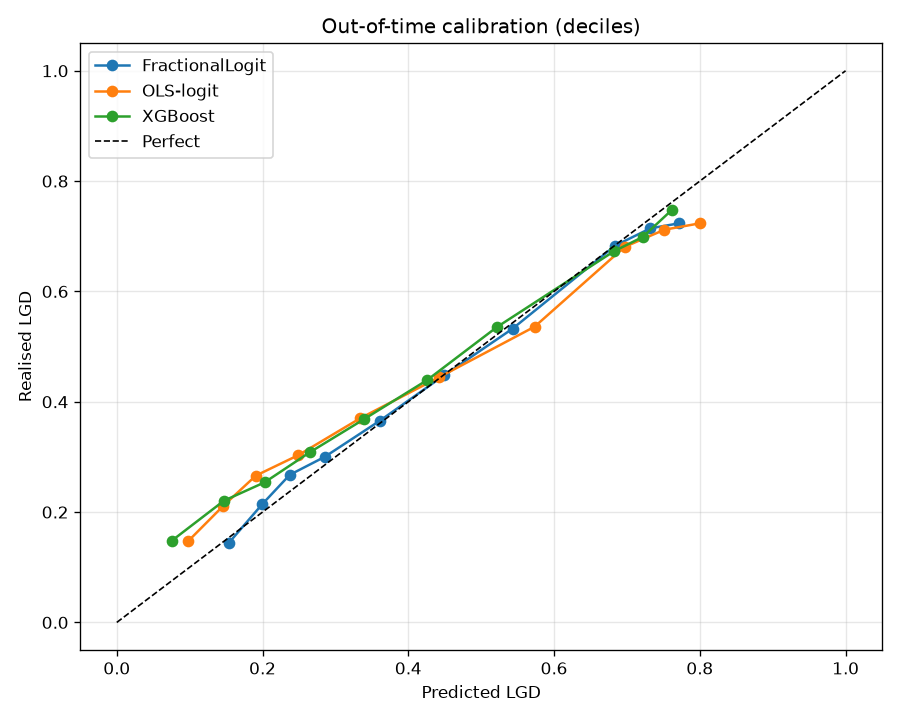
\includegraphics[width=0.85\textwidth]{01_calibration.png}
\caption{Decile calibration of the three models on the OOT cohort.
Fractional logit tracks the diagonal most closely. All three models
underestimate at the highest-LGD decile, driven by rare cases with
negative recoveries (collection costs exceed collateral).}
\end{figure}

\subsection{LGD by collateral type (OOT)}

\begin{figure}[H]
\centering
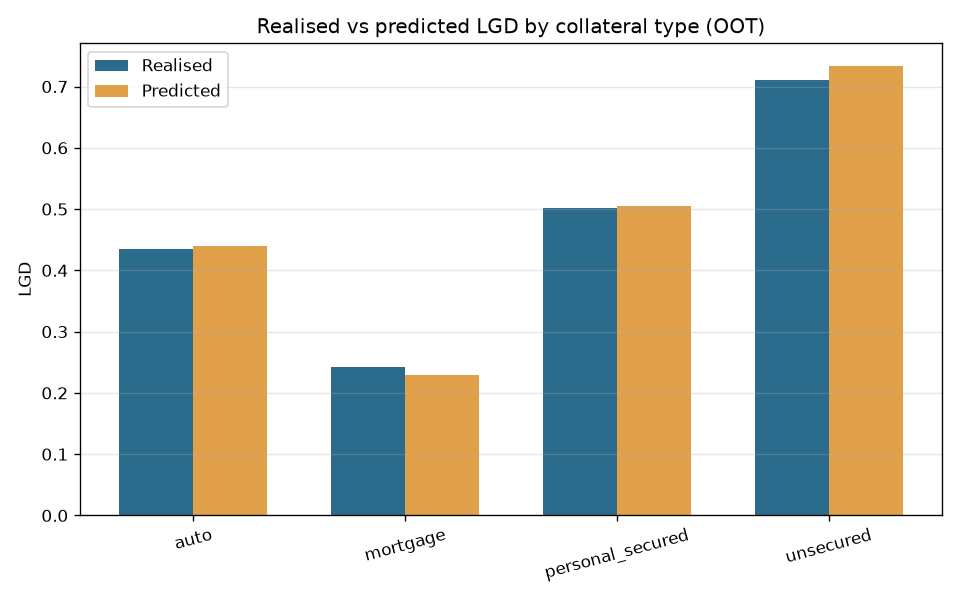
\includegraphics[width=0.75\textwidth]{02_lgd_by_collateral.png}
\caption{Realised versus predicted LGD by collateral type on the OOT
cohort. The model reproduces the collateral-level ordering
(unsecured $\gg$ personal secured $>$ auto $>$ mortgage) with
predicted means within 3\,pp of realised for all four buckets.}
\end{figure}

\subsection{Downturn LGD}

Basel IRB requires LGD estimates to reflect stressed conditions, not
just the long-run average (LRA). One conservative recipe is to take
the 90th percentile of the predicted LGD distribution as the downturn
point estimate per bucket. The uplift is the increment over LRA:

\begin{table}[H]
\centering
\begin{tabular}{l r r r}
\toprule
\textbf{Collateral} & \textbf{LRA LGD} & \textbf{Downturn P90} & \textbf{Uplift} \\
\midrule
Mortgage           & 0.221 & 0.343 & +0.121 \\
Auto               & 0.427 & 0.577 & +0.150 \\
Personal secured   & 0.501 & 0.679 & +0.178 \\
Unsecured          & 0.712 & 0.868 & +0.156 \\
\bottomrule
\end{tabular}
\caption{Downturn-LGD uplift per collateral bucket. Personal secured
carries the largest absolute uplift because its LTV distribution
extends into over-100\% territory, which the model penalises heavily.}
\end{table}

\begin{figure}[H]
\centering
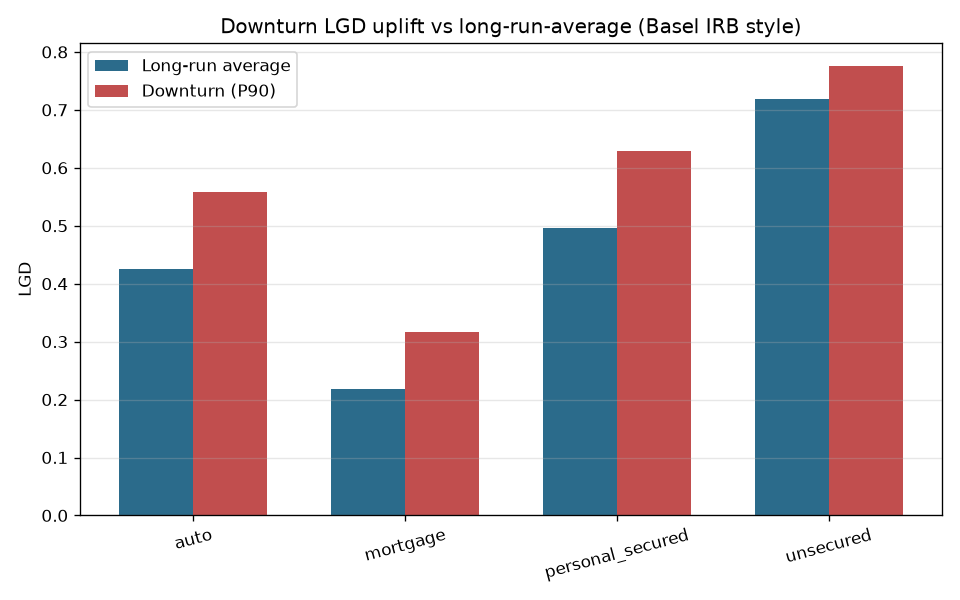
\includegraphics[width=0.75\textwidth]{03_downturn_lgd.png}
\caption{Long-run-average and downturn LGD side-by-side. Downturn
values would be used for regulatory capital and IFRS 9 lifetime ECL
when the forward-looking macro path is stressed.}
\end{figure}

\subsection{Feature importance}

\begin{figure}[H]
\centering
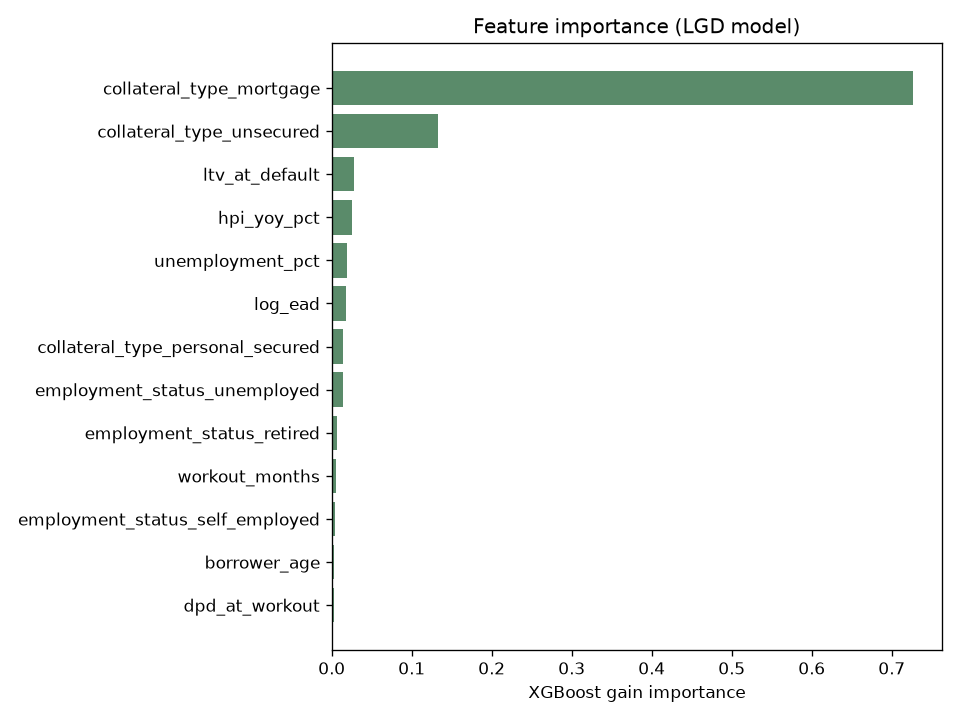
\includegraphics[width=0.8\textwidth]{04_feature_importance.png}
\caption{XGBoost gain-based feature importance. Collateral-type dummies
carry the most signal (as expected: bucket sets the baseline).
Loan-to-value at default and macro variables (HPI, unemployment) are
the strongest continuous predictors.}
\end{figure}

\subsection{Realised LGD distribution}

\begin{figure}[H]
\centering
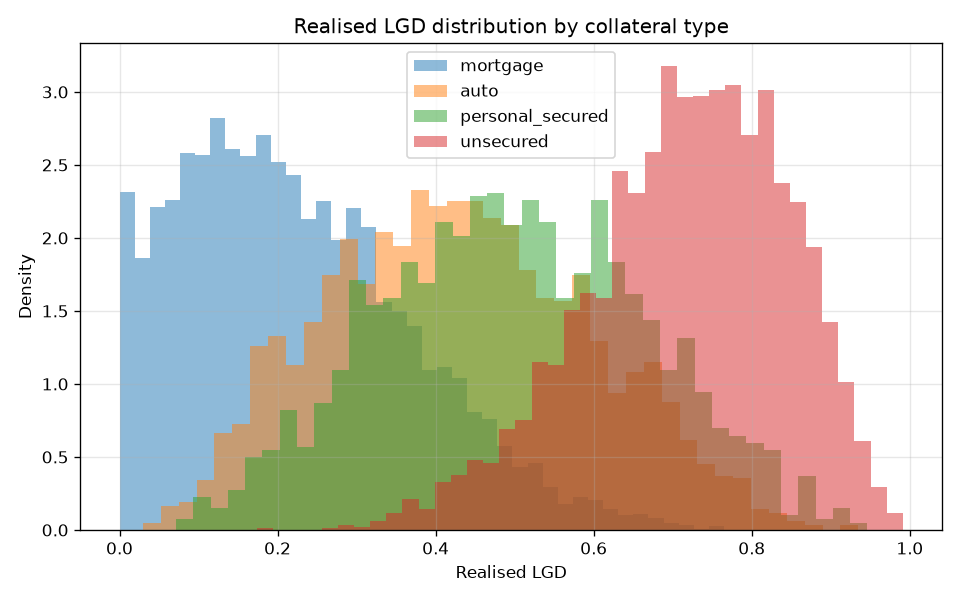
\includegraphics[width=0.85\textwidth]{05_lgd_distribution.png}
\caption{Realised LGD distribution by collateral type. The four
components have visibly different centre and spread. Mortgage
distribution has a heavy left tail (full recovery); unsecured has a
narrow high-LGD peak with almost no full-recovery mass.}
\end{figure}

\subsection{Feature stability (PSI)}

\begin{table}[H]
\centering
\begin{tabular}{l r}
\toprule
\textbf{Feature} & \textbf{PSI (train vs OOT)} \\
\midrule
Unemployment rate    & 17.11 \\
HPI YoY growth       & 17.63 \\
EAD                  & 0.008 \\
LTV at default       & 0.003 \\
Days past due        & 0.003 \\
\bottomrule
\end{tabular}
\caption{PSI between train and out-of-time periods. Macro variables
show very high PSI because the OOT window (2023) has different
macro conditions from the train window (2019--2022, which includes
the pandemic stress). This is by design and does not indicate model
misspecification. Idiosyncratic features are stable.}
\end{table}

The macro-level PSI is the informative half of the story here: it
tells us that the model must be re-estimated or the macro overlay
recalibrated whenever a new macro regime arrives. Idiosyncratic
features are stable across time, which supports the use of the
scorecard on new-vintage originations.

\section{Basel IRB and IFRS 9 fit}

\begin{itemize}
  \item \textbf{Basel IRB LGD requirements:} The scorecard produces
        collateral-level LGD estimates with downturn adjustment via
        the P90 quantile approach. The long-run-average LGD is
        computed on the full train sample which spans a full economic
        cycle (2019--2022), meeting the "sufficient time span"
        requirement.
  \item \textbf{IFRS 9 lifetime LGD:} The macro-conditional feature
        set (unemployment, HPI YoY) allows conditioning the LGD
        estimate on forward-looking macroeconomic scenarios, which is
        how lifetime ECL is generated in stage-2 and stage-3
        classifications.
  \item \textbf{Not fully compliant on:} single-vintage bucket
        granularity may be insufficient for capital calculations that
        require finer risk-driver segmentation; a production model
        would decompose by product family, geography, and origination
        channel.
\end{itemize}

\section{Limitations}

\begin{itemize}
  \item Synthetic data has clean, non-correlated features. Real
        recovery data has heavy dependence on macro cycles, jurisdiction,
        and collateral illiquidity that are only sketched here.
  \item Workout duration is modelled as observed, but in production
        many defaults are still in workout at reporting date and
        require survival modelling for time-to-resolution.
  \item Collateral values at default are treated as observed. In
        reality collateral is re-appraised at workout, and appraisal
        uncertainty is a first-order source of LGD variance.
  \item Downturn P90 is a simple rule. A production model would use a
        macro-conditional simulation to derive the downturn LGD.
\end{itemize}

\section{Files}

\begin{itemize}
  \item \texttt{generate\_data.py} --- synthetic default panel generator
  \item \texttt{train.py} --- three models, calibration, downturn, PSI
  \item \texttt{outputs/} --- metrics, PSI, downturn LGD as CSV
  \item \texttt{figures/} --- five diagnostic plots
\end{itemize}

\end{document}
